%\section{Cautious Adaptation Approach}
%Our approach to cautious adaptation of a defiant component is explained below.



\subsection{Motivating example}

Returning to the example mentioned in the introduction, Figure~\ref{fig:drone_msc} shows high-level message sequence charts (hMSC) specification for the delivery medical payload scenario. Each box in the hMSC corresponds to a basic message sequence chart (bMSC), like UML sequence diagrams, exchanging messages between different entities, while the bMSC are put together through control flows (branches and loops). Figure~\ref{fig:drone_bmsc} depicts the bMSC for the drone delivery example.   
% Need one example bMSC. 

\begin{figure}
    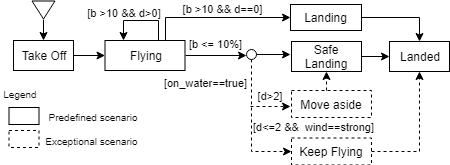
\includegraphics[scale=0.55]{figures/new_drone_msc.png}
    \caption{hMSCs for the drone scenario}
    \label{fig:drone_msc}
\end{figure}

\begin{figure}
    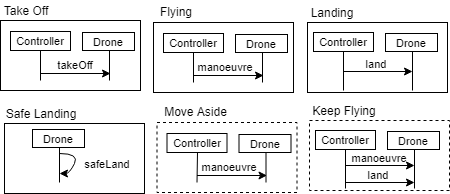
\includegraphics[scale=0.5]{figures/new_drone_bmsc.png}
    \caption{bMSCs for the drone delivery scenario}
    \label{fig:drone_bmsc}
\end{figure}

In the hMSC of Figure~\ref{fig:drone_msc}, the pre-defined scenarios, represented by a full rectangle, are part of the normal specification of the drone. Thus, the pilot, via a controller, can make the drone taking off, then keeps manoeuvring it where the battery is above the threshold $\theta = 10\%$  and it does not reach the expected location. When it does, then the pilot send a landing command to the drone, which acknowledge when landed in the ground.  During the flight, the drone periodically checks the status of its internal components, such as battery level and distance from the destination, represented by \textit{b} and \textit{d}, respectively, in the conditions over the hMSC transitions. In the example, if the battery level is below the threshold, then the drone reports the controller its data, otherwise it performs a safe landing by itself, since this is according to its predefined specification. 

However, the pilot knows that, if the distance from the expected landing pad is less than 1km and the drone is flying over the river (condition \textit{on\_water==true}), then he/she can keep the drone flying even in a low-level battery situation and then land it, thus being able to complete its overall goal (delivering the medical payload) successfully. Nonetheless, if the battery is low, the drone is above water, but the drone is more than 2km away, then necessary action is to move the drone aside in order to make it land on the ground. We represent those exceptional scenarios graphically by a dashed rectangle.  

We extend the MSC specification with the operator (o), which represents an \textit{interception point} in which exceptional scenarios can be plugged in to enable  wrapping the defiant behaviour of the drone. Note that more exceptional behaviours could be plugged in the same injection point indicating another possible behaviours according to other contextual information. If there is no exceptional scenario plugged in the injection point, then the expected behaviour is performed.

%In order to analyse this strategy, we transform the scenario specification into LTS models for each component, and then compose them in parallel to obtain the global behaviour of the system, as in~\cite{Uchitel:2003}. To do so, we need to introduce a special internal transition to represent the late decision on what would be the runtime behaviour of the defiant component. For instance, the first model shown in Figure~\ref{fig:drone_lts} (CONTROLLER\textunderscore DRONE) illustrates the LTS for the composition of the drone and the controller components in which a transition called \textit{decision} is introduced (from state 5 to 6) to indicate the injection point. See that, the next action after \textit{decision} is \textit{safeLanding}, i.e., if no exceptional scenario is plugged, then the component follows its ordinary behaviour.    

%The second model of Figure~\ref{fig:drone_lts} represents the model of the exceptional scenario, which we called as WRAPPER. Note that it contains the \textit{decision} action to synchronize with the its counterpart in the previous model, but after \textit{decision} is reached, the Wrapper changes the behaviour to keep the drone flying and, after, landing. This can be seen in the composition model of the system (controller and drone) and the wrapper, which is represented by model S in Figure~\ref{fig:drone_lts}. Therefore, the composition with the wrapper avoided the drone of performing its defiant behaviour.    

%\begin{figure}
%    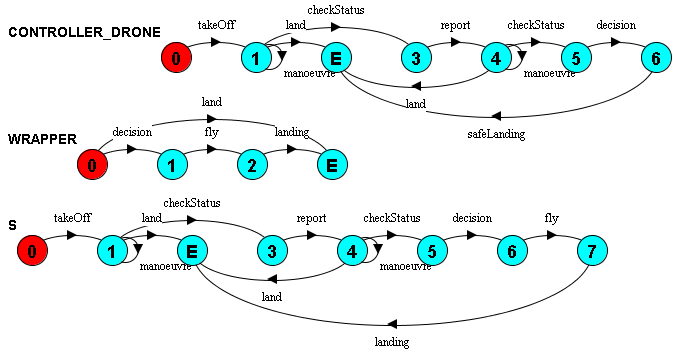
\includegraphics[scale=0.55]{figures/wrapper_lts.png}
%   \caption{LTS behaviour for drone and wrapper components }
%    \label{fig:drone_lts}
%\end{figure}

